\chapter{Probabilistic Models} \label{chap:models}

\section*{}

\section{Introduction}

Probabilistic or statistical models represent explicit assumptions about a 
problem domain, in the form of a model. This model usually encompasses random 
variables\footnote{Variable whose value is given by a probability distribution, 
commonly represented by $\Theta$.}, in the form of probability distributions, 
and the relation and dependence between the variables.~\cite{Winn2013}

In the following sections we describe a common way to represent probabilistic models, probabilistic graphical models (PGM) or, simply, graphical models.

\section{Probabilistic Graphical Models}

A PGM is a graph based model where the nodes represent random variables and the 
(directed or undirected) edges represent a conditional dependence between 
variables. An example is shown in figure~\ref{fig:pgm}.

\begin{figure}[h]
	\begin{center}
		\leavevmode
		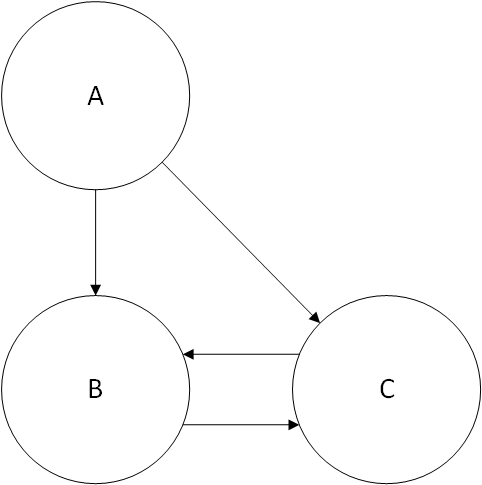
\includegraphics[width=0.36\textwidth]{pgm}
		\caption{Example of a PGM: B and C depend on A, B depends on C and C depends on B. }
		\label{fig:pgm}
	\end{center}
\end{figure}

PGMs and their extensions, where we show some examples of them in the following 
sections, are exceptionally well suited for reasoning and to reach conclusions 
based on available information (both domain expert and data), even in the 
presence of uncertainty. PGMs provide a general framework that allows 
representation, inference and learning on these 
models.~\cite{koller2009probabilistic}

There is extensive research and available literature in this area. Some notable 
examples include, but are not limited to, the books \textit{"Probabilistic 
Graphical Models: Principles and Techniques"} by Daphne Koller and Nir 
Friedman~\cite{koller2009probabilistic} and \textit{"Pattern Recognition and 
Machine Learning"} (Chapter 8: Graphical Models) by Christopher 
Bishop~\cite{bishop2006pattern}. It is also worth mentioning that there is a 
MOOC \footnote{Massive Open Online Course} named \textit{"Probabilistic 
Graphical Models"}, also by Daphne Koller (Stanford), freely available on 
Coursera \footnote{https://www.coursera.org/course/pgm}.

In the following sections, we describe three important categories of graphical 
models: Bayesian networks, Markov random fields and its extension to hidden 
Markov models. There are plenty of other graphical models however they were 
deemed not relevant enough to be included in this literature review.

\section{Bayesian Networks}

Bayesian networks, also named directed graphical models, is a type of PGM where 
the edges in the graph representation are directed and represent causal 
relationships between random variables or group of random variables (see figure 
\ref{fig:pgm}). This concept was first introduced by Pearl in 
1985~\cite{Pearl1985}, which uses Bayes' conditioning~\cite{bayes1763essay} as 
the basis for updating information.

Bayesian networks follow the Bayesian approach to statistics and probabilities. 
In contrast to classical or physical probability, Bayesian probability (of an 
event) is a person's \textit{degree of belief} in that event 
~\cite{Heckerman1996}. While it may seen that a degree of belief is somewhat 
arbitrary or may lack precision and accuracy, multiple 
authors~\cite{Ramsey1931, Tversky1974, Shachter1988} argue that small 
variations in probability do not have a big influence in the decision making 
process and that measuring beliefs lead to the same rules of probability (which 
can be summarized with the product rule \ref{eq:product} and the sum rule 
\ref{eq:sum}~\cite{MacKay2005}). 

\begin{equation}
P(x, y \mid \mathcal{H}) = P(y \mid x, \mathcal{H}) P(x \mid \mathcal{H}) 
\footnote{$\mathcal{H}$: hypotesis or assumptions the probabilities are based} 
\label{eq:product}
\end{equation}

\begin{equation}
P(x, \mathcal{H}) = \sum_{y}^{} P(x \mid y, \mathcal{H}) P(y \mid \mathcal{H}) 
\label{eq:sum}
\end{equation}

Formally \cite{Pearl:1988:PRI:534975}, a Bayesian network $ B $ represents a 
joint probability distribution (JPD) over a set of variables $ \mathbf{U}$ and 
can be defined by a pair $ B = \langle G, \Theta \rangle $. $ B $ is a DAG 
(directed acyclic graph) where the vertices represent the random variables $ 
X_{1}, ..., X_{n} $. $ \Theta $ represents the set of parameters that quantify 
the network. For each possible value $ x_{i} $ of $ X_{i} $, and $ 
\prod_{x_{i}} $ of $ \prod_{X_{i}} $ (set of parents of $ X_{i} $ in $ G $), it 
contains a parameter $ \theta_{x_{i} \mid \prod_{x_{i}}} = P_{B}(x_{i} \mid 
\prod_{x_{i}}) $. Therefore, the JPD can be defined as

\begin{equation}
P_{B}(X_{1}, ..., X_{n}) = \prod_{i=1}^{n} P_{B}(X_{i} \mid 
\prod\nolimits_{X_{i}}) =
\prod_{i=1}^{n} \theta_{X_{i} \mid \prod_{X_{i}}} \label{eq:jpd}
\end{equation}

which expresses the factorization properties of the JPD. \cite[section 
8.1.]{bishop2006pattern} goes in detail on how to apply the eq \ref{eq:jpd}.

These properties of Bayesian networks make it an excellent tool for expressing 
causal relationships. Heckerman~\cite{Heckerman1996} lists multiple advantages 
of Bayesian networks on modelling and data analysis: ``readily handles 
situations where some data entries are missing'', ``gain understanding about a 
problem domain and to predict the consequences of intervention'', ``ideal 
representation for combining prior knowledge and data'' and ``efficient and 
principled approach for avoiding the overfitting of data''.

Regarding the area of e-commerce specifically, some research has been done 
where Bayesian networks are applied. \cite{Nasambu2014} is an attempt at 
predicting sales in e-commerce using social media data. \cite{Moe2002} also 
proposes a Bayesian based model to predict online purchasing behaviour using 
navigational clickstream data.

\section{Markov Random Fields}

\section{Hidden Markov Models}

\cite{Rabiner1989}

\section{Summary}
